% Template for ICIP-2018 paper; to be used with:
%          spconf.sty  - ICASSP/ICIP LaTeX style file, and
%          IEEEbib.bst - IEEE bibliography style file.
% --------------------------------------------------------------------------
\documentclass{article}
\usepackage{spconf,amsmath,graphicx}
%\usepackage[subsection]{placeins}
\usepackage[section]{placeins}
\usepackage{listings}
\lstset{
  basicstyle=\sffamily,
  columns=fullflexible,
  frame=single,
  breaklines=true,
  postbreak=\mbox{\textcolor{}{$\hookrightarrow$}\space},
}

% Example definitions.
% --------------------
\def\x{{\mathbf x}}
\def\L{{\cal L}}
\def\listingsfontinline{\ttfamily}

% Title.
% ------
\title{Image Processing Assignment-1}
%
% Single address.
% ---------------
\name{M.Arun kumar}
\address{173079004}
%
% For example:
% ------------
%\address{School\\
%	Department\\
%	Address}
%
% Two addresses (uncomment and modify for two-address case).
% ----------------------------------------------------------
%\twoauthors
%  {A. Author-one, B. Author-two\sthanks{Thanks to XYZ agency for funding.}}
%	{School A-B\\
%	Department A-B\\
%	Address A-B}
%  {C. Author-three, D. Author-four\sthanks{The fourth author performed the work
%	while at ...}}
%	{School C-D\\
%	Department C-D\\
%	Address C-D}
%
\begin{document}
%\ninept
%
\maketitle
%
\begin{abstract}
I have developed tool to perform the basic intensity transformation on the Images. Images here can be grey scale or color but only images of the type png,jpeg,jpg,xmp are accepted as input. Intensity transforms that can be performed on this images using the tool are Histogram Equalization, Gamma transform, Log transform, Blurring Image, Sharpening Image and Edge detection using Sobel operators is added as the additional transform. All of these transforms are applied on some of the images and the results are shown in this report.
\end{abstract}

\section{Introduction}
\label{sec:intro}
Main idea behind this tool is to implement various transformation techniques on any of the image.Images can be of many types like color, grey scale etc. Different Images have different underlying data representations like color images can be represented with 3 arrays if the pixel intensities are represented in RGB format, Same image if represented in HSV format will have arrays corresponding to H,S,V respectively each array element will be the value of Hue,Saturation and Value. Similarly grey scale  is one in which the value of each pixel represents intensity information. This tool will convert any image given to it into its HSV data and performs all the operations on the Intensity(V) array and then merge it with the original Hue(H) and Saturation(S) arrays to get back the original image. 


\section{Background read}
\label{sec:format}
This tool is implemented using Python\cite{WEBSITE:10}. I have used PyQt4\cite{WEBSITE:9} binding for implementing GUI it runs on Windows, Linux, Mac OS X and various UNIX platforms. It does not support Android and iOS. To handle color and grey scale images opencv\cite{WEBSITE:4} library is used. Any image uploaded will be considered as color image and its HSV arrays\cite{WEBSITE:2} are extracted. To perform operations on the Intensity values numpy\cite{WEBSITE:1} library is used  


\section{Approach}
\label{sec:pagestyle}
Apart from transformations there are some file handling and operation control features in this tool. Every operation is associated with a button or scroll bar(only for sharpening image). Each button in turn when clicked calls the corresponding method to perform the operation on the image. Before any change is made to the data it is stored in a global variable so that the Undo functionality can be implemented easily. Each of the transform that is implemented by this tool and approach followed to implement it is listed below
\subsection{Histogram Equalization}
Histogram equalization\cite{WEBSITE:4} is implemented by taking the CDF of the pixel intensities, for each intensity level number of such pixels in the image are found and this result is stored in a variable(CDF) and it is updated for every intensity level by adding the previous value also the new intensity is calculated by dividing it with the size of the image and then multiplying it with maximum intensity i.e.,255.
\subsection{Gamma transform}
Each intensity value of the original image is normalized and raised to the power of $1/gamma$ given by the user this result is multiplied with a constant value to return the intensity range of the original image. In this tool constant for gamma transform\cite{WEBSITE:12} is chosen to be 255.So if the user gives gamma to be less than 1 all the intensity values are reduced and the image appears darker. Similarly if gamma is greater than 1 image appears brighter.
\subsection{Log transform}
Each intensity value of the original image is multiplied by a constant and log of that value is taken as new intensity. In this tool constant for log transform is chosen to be 46 because the intensity range from images is from 0 to 255. log of these values would result in values from 0 to 5.54 to keep the range of intensities same constant is chosen to be 46.
\subsection{Blurring Image}
To blur an image blurring kernel is used. Gaussian kernel is used and the window size of the kernel is determined by the sigma(variance) value given by the user larger the sigma value more blurring happens and vice-verse. After sigma is taken from the user kernel of size $(2*sigma,2*sigma)$ is formed and the image is convolved with the filter(kernel) to get the blurred image. 

\subsection{Sharpening Image}
To Sharpen an image kernel is used. Laplacian kernel is used and the window size of the kernel $(3,3)$ is formed and the image is convolved with the image to get the sharpened image. Extent of sharpening is controlled with the scroll bar minimum value of the scroll bar is 1 and maximum is 10. If scroll bar is set to 1 the resultant image is the sum of original image and convolved image. Similarly if the scroll bar is set to 10 the resultant image is sum of the original image and 10 times the convolved image.

\subsection{Sobel operators(Horizontal and vertical edge detection)}
To detect edges kernel is used. Here Sobel kernel is used and the window size of the kernel $(3,3)$ is formed and the image is convolved with the image to get the sharpened image. Two kernels are used to detect 2 edges (horizontal and vertical) and the result of both of them is added to display the horizontal and vertical edges.

\section{Selection of test images}
\label{sec:typestyle}

Following are the images used for testing the various transformation techniques.
\subsection{Histogram Equalization}
\begin{figure}[htb]

\begin{minipage}[b]{1.0\linewidth}
  \centering
  \centerline{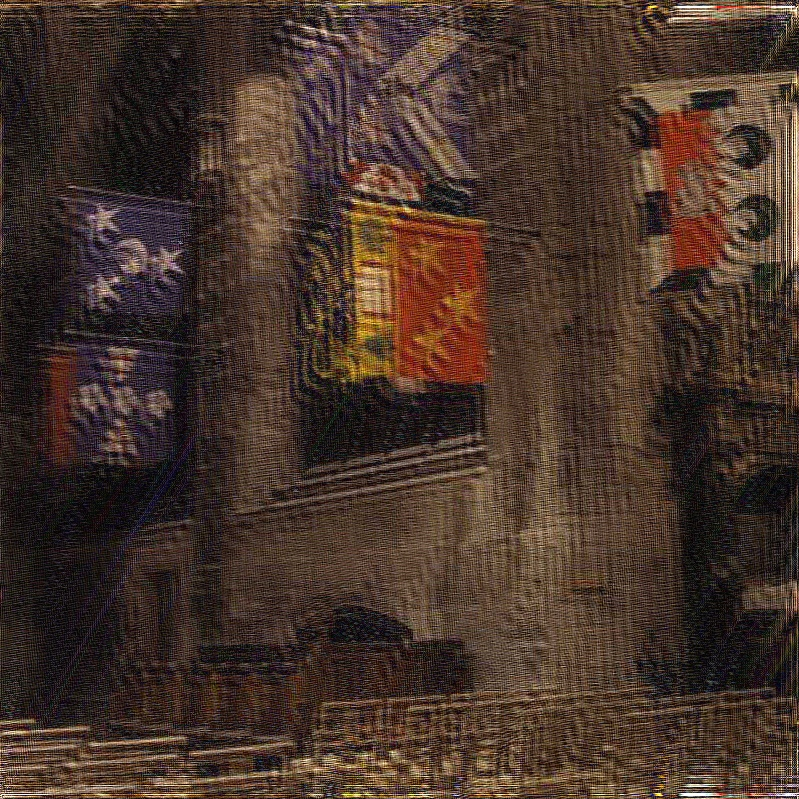
\includegraphics[width=8.5cm]{temp.jpg}}
%  \vspace{2.0cm}
  \centerline{Test image for Histogram equalization\cite{WEBSITE:13}}\medskip
\end{minipage}
%
\end{figure}
This is image is chosen for histogram equalization because its Histogram is more skewed towards low intensity levels. Results of histogram equalisation will be clearly visible with this image. 

\subsection{Gamma Correct}
\begin{figure}[htb]

\begin{minipage}[b]{1.0\linewidth}
  \centering
  \centerline{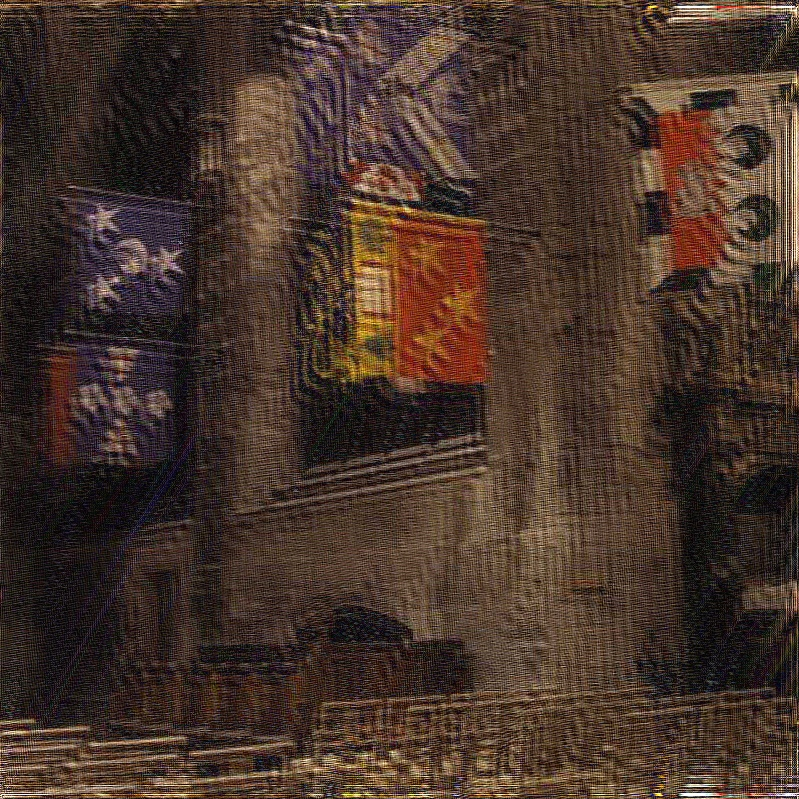
\includegraphics[width=8.5cm]{temp.jpg}}
%  \vspace{2.0cm}
  \centerline{Test image for Gamma correction\cite{WEBSITE:12}}\medskip
\end{minipage}
%
\end{figure}
This is image is chosen for Gamma correction because it is brighter image and the effect of gamma transform for different gamma values can be clearly observed.

\subsection{Log Transform}
\begin{figure}[htb]

\begin{minipage}[b]{1.0\linewidth}
  \centering
  \centerline{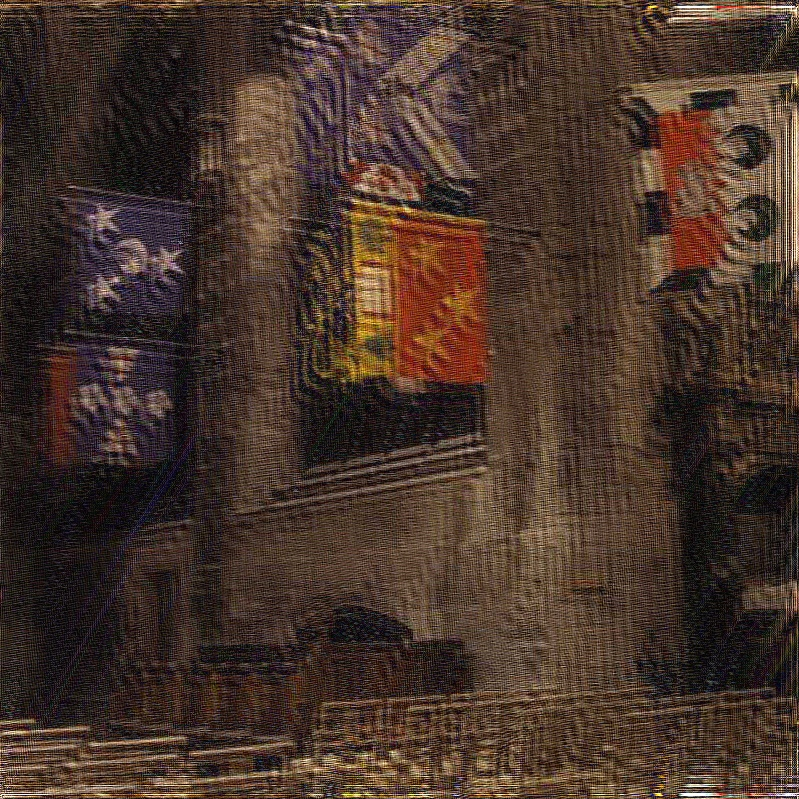
\includegraphics[width=8.5cm,height=7cm,keepaspectratio]{temp.jpg}}
%  \vspace{2.0cm}
  \centerline{Test image for Log Transform\cite{WEBSITE:16}}\medskip
\end{minipage}
%
\end{figure}
Effect of Log transformation is more clearly visible in Grey scale image, So grey scale image is chosen for testing Log transformation. 

\subsection{Blur Image}
\begin{figure}[htb]

\begin{minipage}[b]{1.0\linewidth}
  \centering
  \centerline{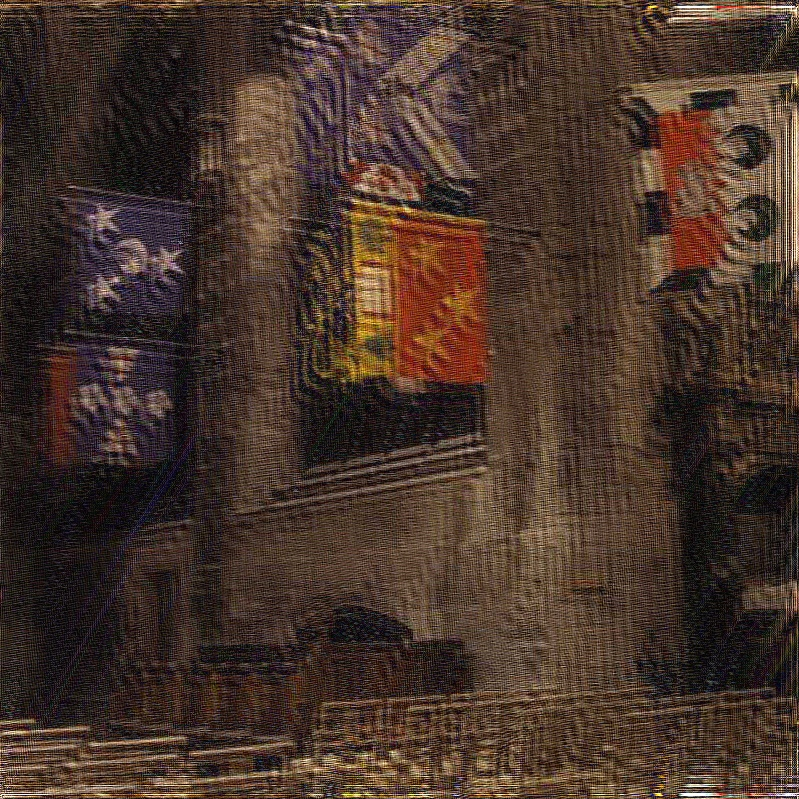
\includegraphics[width=8.5cm,height=5cm,keepaspectratio]{temp.jpg}}
%  \vspace{2.0cm}
  \centerline{Test image for Blurring\cite{WEBSITE:14}}\medskip
\end{minipage}
%
\end{figure}
Any image can chosen for blurring image but image which has more details in it will give the best output so this image is chosen. 


\subsection{Sharpen Image}
\begin{figure}[htb]

\begin{minipage}[b]{1.0\linewidth}
  \centering
  \centerline{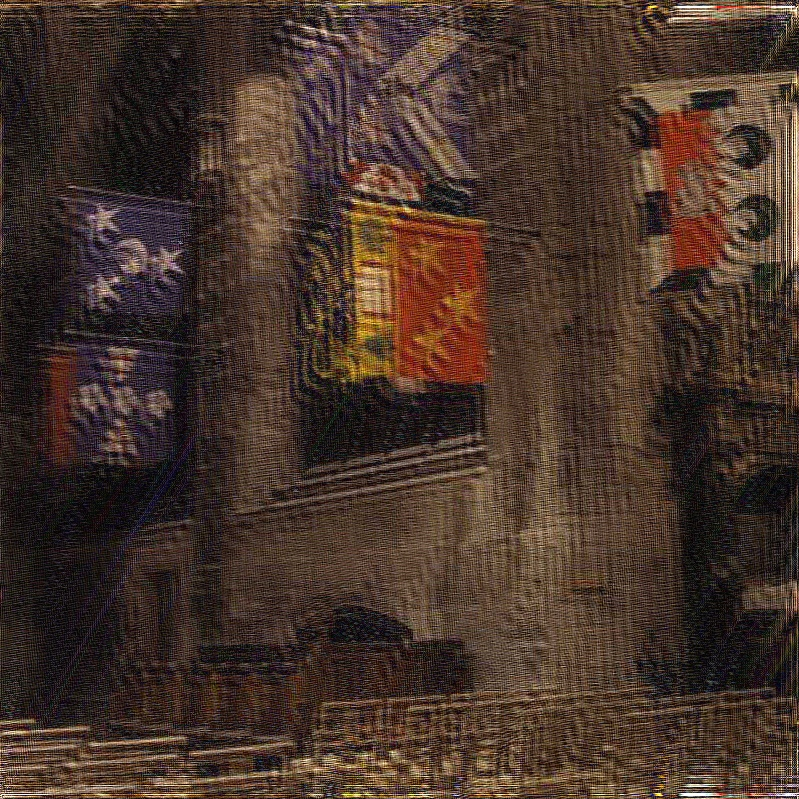
\includegraphics[width=8.5cm,height=4cm,keepaspectratio]{temp.jpg}}
%  \vspace{2.0cm}
  \centerline{Test image for Sharpening\cite{WEBSITE:17}}\medskip
\end{minipage}
%
\end{figure}

 
\subsection{Sobel operation}

\begin{figure}[htb]

\begin{minipage}[b]{1.0\linewidth}
  \centering
  \centerline{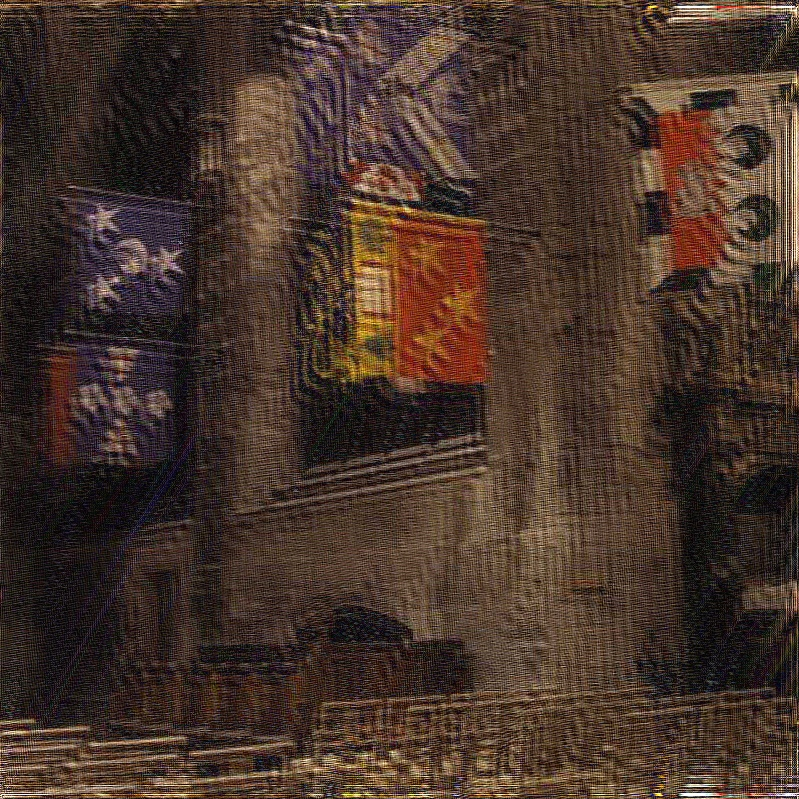
\includegraphics[width=8.5cm,height=5cm,keepaspectratio]{temp.jpg}}
%  \vspace{2.0cm}
  \centerline{Test image for Sobel opeartion\cite{WEBSITE:15}}\medskip
\end{minipage}
%
\end{figure}
Image which has more horizontal and vertical edges will be required since Sobel operators for detecting horizontal and vertical edges is used as kernel

\section{Results on Test Images}
\label{sec:print}

Following are the images after appying various transformation techniques.
\subsection{Histogram Equalization}
\begin{figure}[htb]

\begin{minipage}[b]{1.0\linewidth}
  \centering
  \centerline{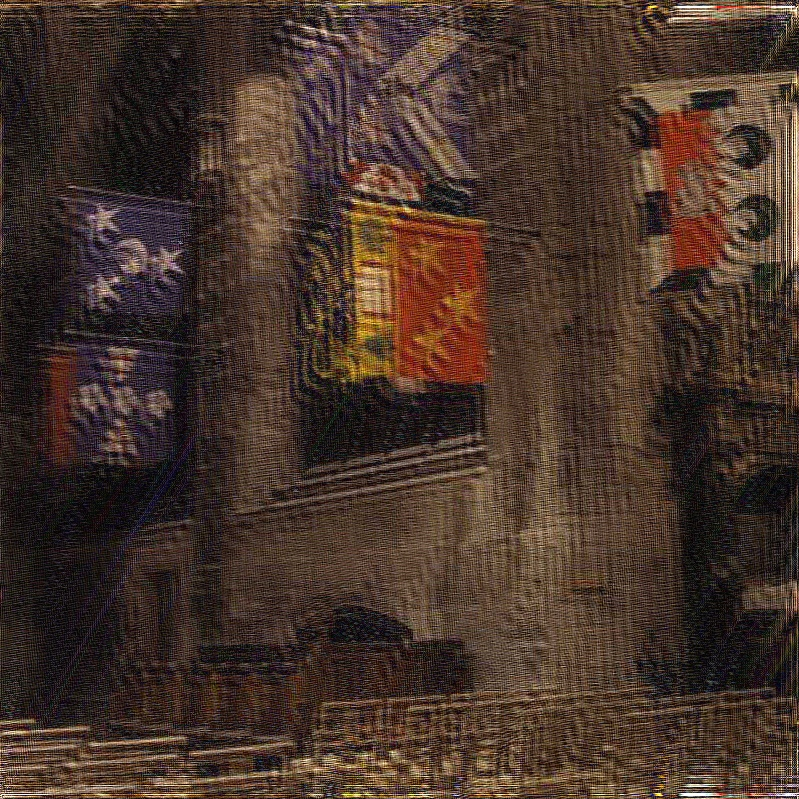
\includegraphics[width=8.5cm]{temp.jpg}}
%  \vspace{2.0cm}
  \centerline{Test image after applying Histogram equalization}\medskip
\end{minipage}
%
\end{figure}


\subsection{Gamma Correct}
\subsubsection{gamma = 0.1}
\begin{figure}[htb]

\begin{minipage}[b]{1.0\linewidth}
  \centering
  \centerline{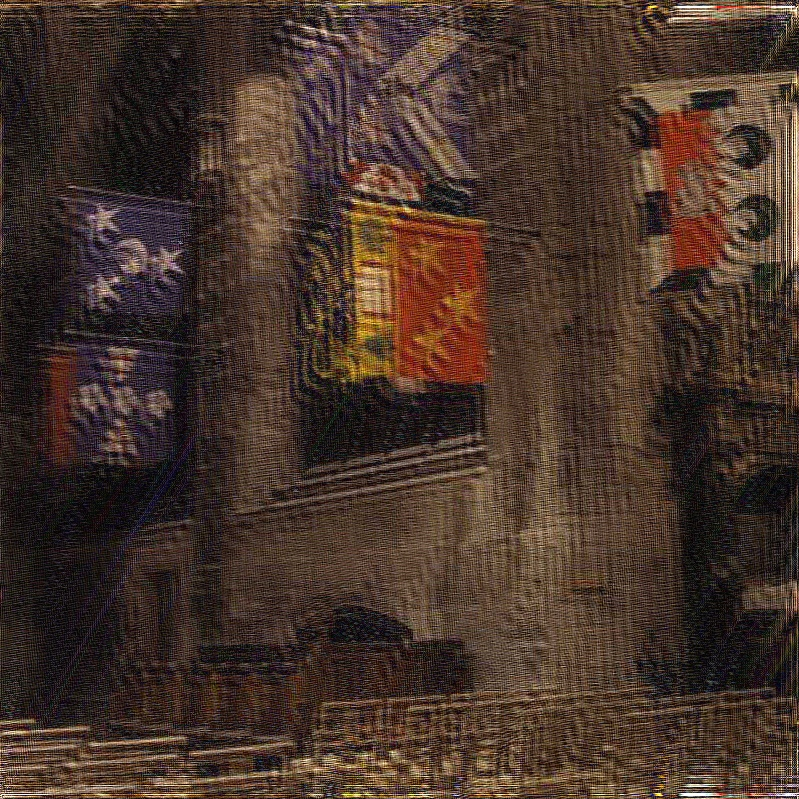
\includegraphics[width=8.5cm,height=6cm,keepaspectratio]{temp.jpg}}
%  \vspace{2.0cm}
  \centerline{Test image after applying Gamma correction with gamma = 0.1}\medskip
\end{minipage}
%
\end{figure}
\subsubsection[h]{gamma = 2.2}Image after applying gamma transform 
\begin{figure}[h]

\begin{minipage}[b]{1.0\linewidth}
  \centering
  \centerline{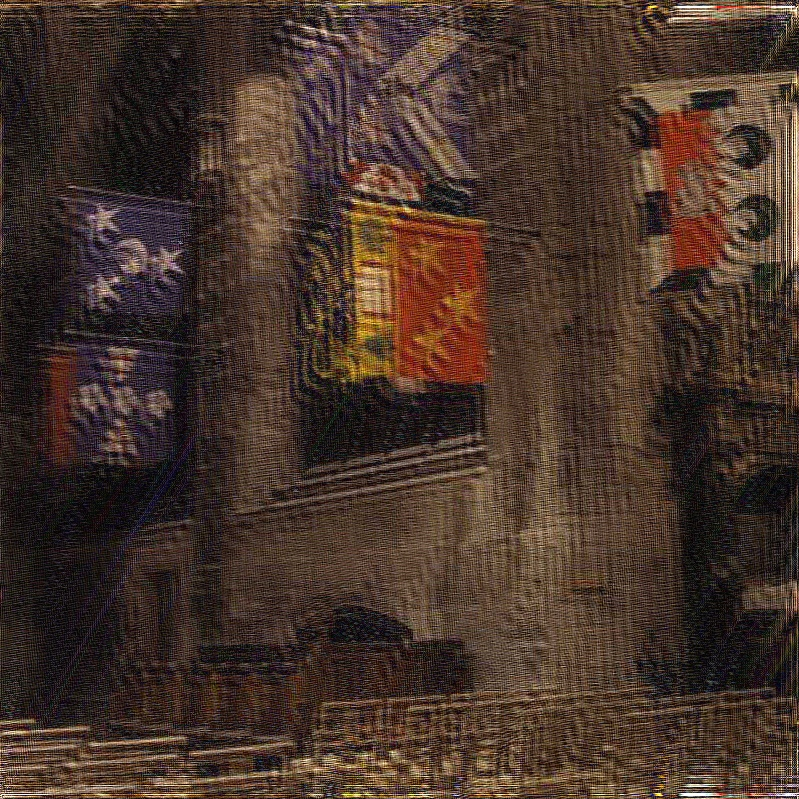
\includegraphics[width=8.5cm]{temp.jpg}}
%  \vspace{2.0cm}
  \centerline{Test image after applying Gamma correction with gamma = 2.2}\medskip
\end{minipage}
%
\end{figure}


\subsection[h]{Log Transform}
\begin{figure}[!h]

\begin{minipage}[b]{1.0\linewidth}
  \centering
  \centerline{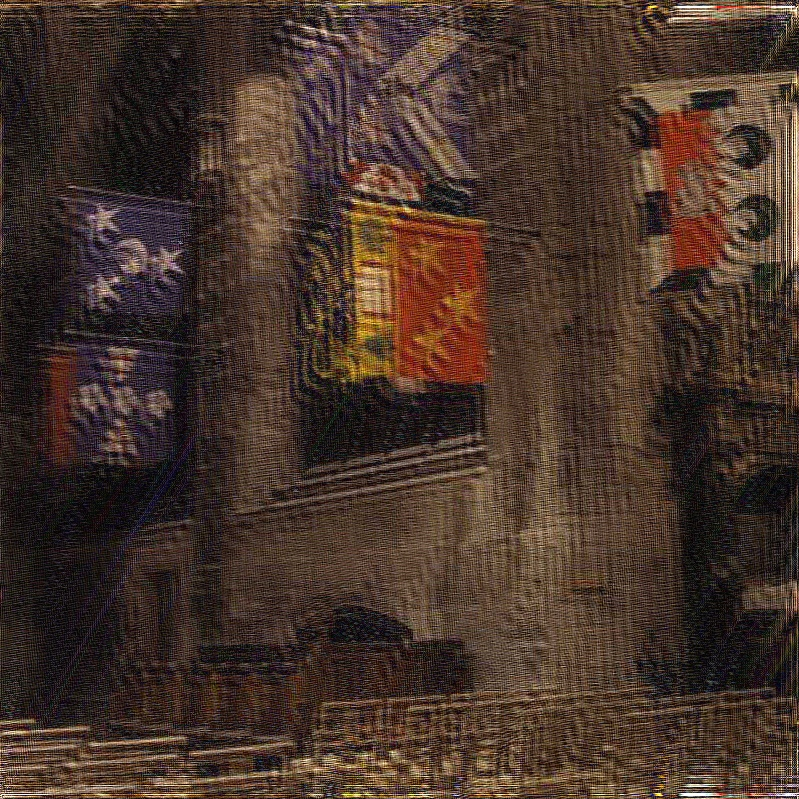
\includegraphics[width=8.5cm]{temp.jpg}}
%  \vspace{2.0cm}
  \centerline{Test image after applying Log Transform}\medskip
\end{minipage}
%
\end{figure}


\subsection[h]{Blur Image}Results of blurring with different Gaussian kernels 
\subsubsection[h]{Blur using Gaussian kernel with variance 5 }
\begin{figure}[htb]

\begin{minipage}[b]{1.0\linewidth}
  \centering
  \centerline{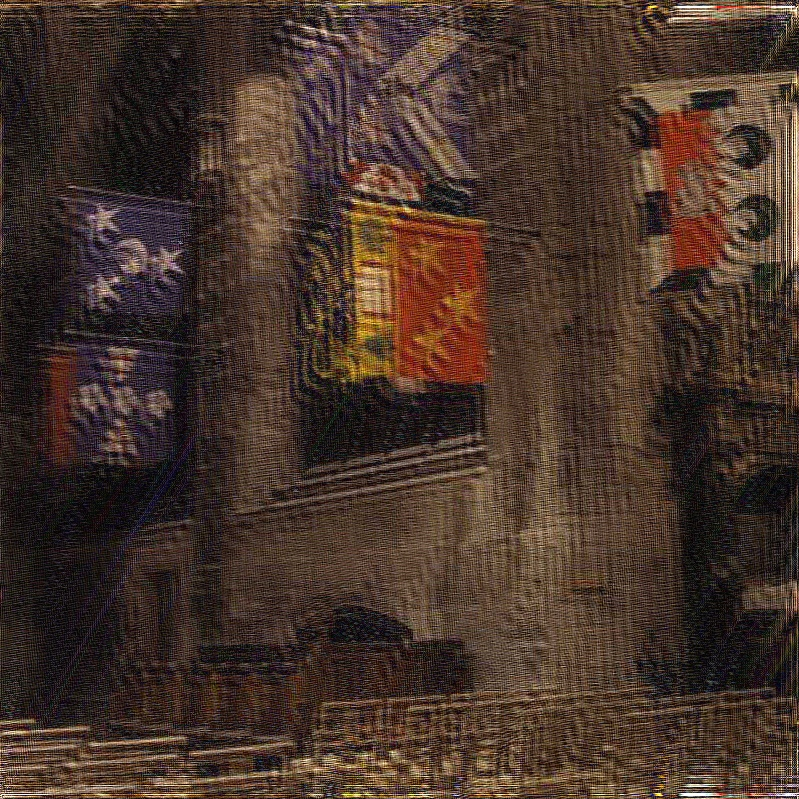
\includegraphics[width=8.5cm,height = 5cm ,keepaspectratio]{temp.jpg}}
%  \vspace{2.0cm}
  \centerline{Test image after Blurring with Gaussian kernel with variance 5}\medskip
\end{minipage}
%
\end{figure}
\subsubsection[h]{Blur using Gaussian kernel with variance 20}
\begin{figure}[h]

\begin{minipage}[b]{1.0\linewidth}
  \centering
  \centerline{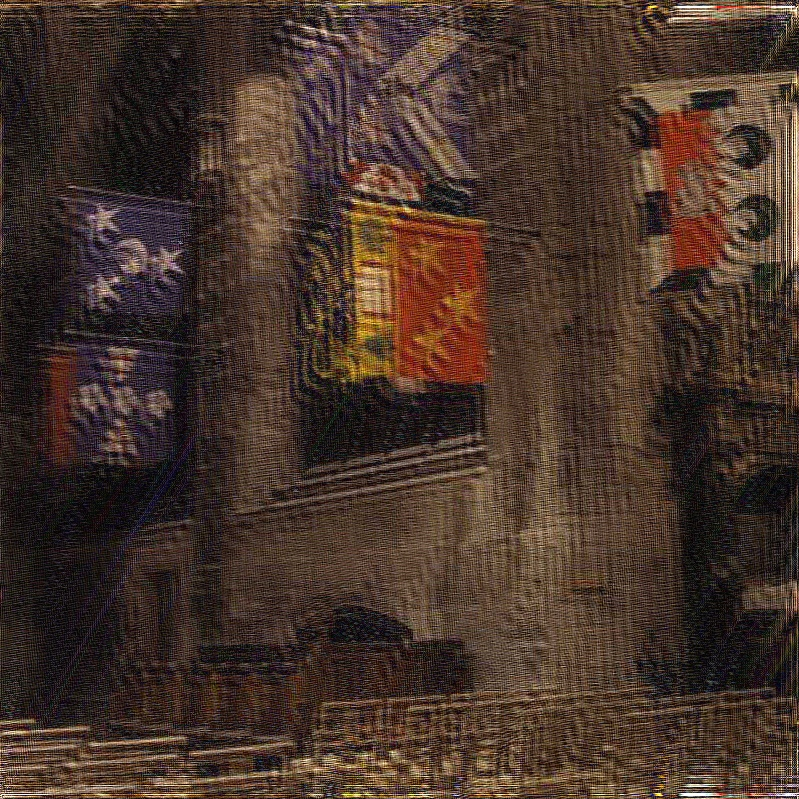
\includegraphics[width=8.5cm,height = 5cm ,keepaspectratio]{temp.jpg}}
%  \vspace{2.0cm}
  \centerline{Test image after Blurring with Gaussian kernel with variance 20}\medskip
\end{minipage}
%
\end{figure}


\subsection[h]{Sharpen Image}Result after applying Laplacian $(3,3)$ kernel
\begin{figure}[h]

\begin{minipage}[b]{1.0\linewidth}
  \centering
  \centerline{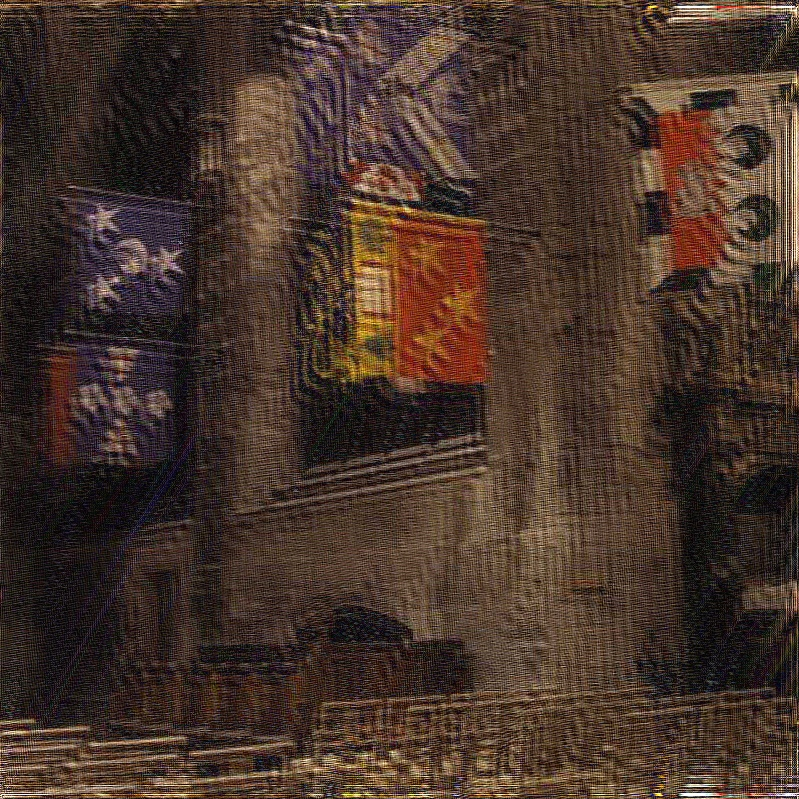
\includegraphics[width=8.5cm,height =4cm ,keepaspectratio]{temp.jpg}}
%  \vspace{2.0cm}
  \centerline{Test image after applying sharpening filter}\medskip
\end{minipage}
%
\end{figure}

 
\subsection[h]{Sobel operation}Result of applying Sobel kernel to detect horizontal and vertical edges. Here the test image is convolved with the kernel to detect horizontal edges at the same time another kernel is applied to the test image to detect vertical edges to detect vertical edges. Result of the convolution of these is added to get the horizontal and vertical edges in image

\begin{figure}[htb]

\begin{minipage}[b]{1.0\linewidth}
  \centering
  \centerline{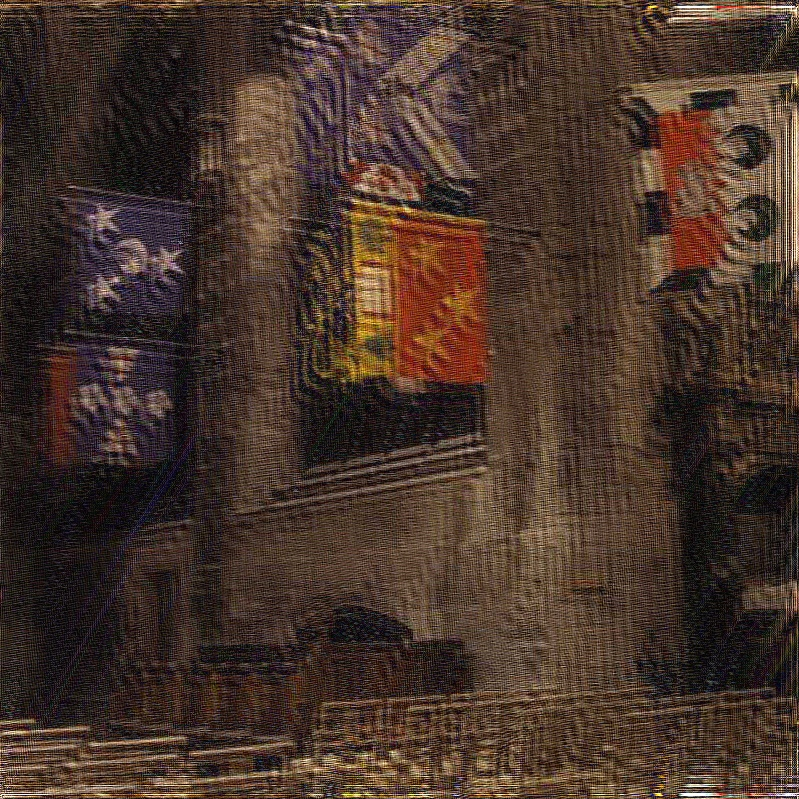
\includegraphics[width=8.5cm]{temp.jpg}}
%  \vspace{2.0cm}
  \centerline{Test image after applying Sobel operator}\medskip
\end{minipage}
%
\end{figure}






\section{Disscussion}
\label{sec:ref}

Main problem faced during development is choice of language. I got to know that Matlab has a drag and drop type of making GUI, but it is licensed i wanted to work with open source. The choice I was left with was c++ and python. I was not well versed in both of them. Since python syntax is easy i chose python. Implementation of  GUI created a lot of problems I did not know which python binding to use, after searching online and found that tkinter is the basic and primitive binding in python so i chose that and started working with it but after spending entire day on it nothing much was happening so i shifted to pyqt after finding a tutorial\cite{WEBSITE:9} on pyqt and completed the GUI part using pyqt. For image operations Opencv \cite{WEBSITE:3}and numpy\cite{WEBSITE:1} libraries are used though it was not easy documentation is available online.

 If more time was given i would have implemented convolution using vectors to reduce the computations and GUI also can improved by  making the window responsive adding short cuts to all the operations etc.,

% References should be produced using the bibtex program from suitable
% BiBTeX files (here: strings, refs, manuals). The IEEEbib.bst bibliography
% style file from IEEE produces unsorted bibliography list.
% -------------------------------------------------------------------------
\bibliographystyle{IEEEbib}
\bibliography{strings,refs}
\onecolumn
\section{APPENDIX}
\lstinputlisting[language=Python]{assignment2.py}
\end{document}
